\documentclass[a4paper]{article}
\usepackage[utf8]{inputenc}
\setcounter{tocdepth}{3}
\usepackage{setspace}
\usepackage{graphicx}
\usepackage{caption}
\usepackage{subcaption}
\usepackage{amsmath}
\usepackage{amssymb,wasysym}
\usepackage{wrapfig}
\usepackage{fancyhdr} 
\usepackage{hyperref}
 %%%%%%%%%%%%%%%%%%%%%%%%%%%%%%%%%%%%%%%%%%%%%%%%%%%%%%%%%%%%%%%%%%%%%%%%%%%%%%%% 
%%% ~ Arduino Language - Arduino IDE Colors ~                                  %%%
%%%                                                                            %%%
%%% Kyle Rocha-Brownell | 10/2/2017 | No Licence                               %%%
%%% -------------------------------------------------------------------------- %%%
%%%                                                                            %%%
%%% Place this file in your working directory (next to the latex file you're   %%%
%%% working on).  To add it to your project, place:                            %%%
%%%     %%%%%%%%%%%%%%%%%%%%%%%%%%%%%%%%%%%%%%%%%%%%%%%%%%%%%%%%%%%%%%%%%%%%%%%%%%%%%%%% 
%%% ~ Arduino Language - Arduino IDE Colors ~                                  %%%
%%%                                                                            %%%
%%% Kyle Rocha-Brownell | 10/2/2017 | No Licence                               %%%
%%% -------------------------------------------------------------------------- %%%
%%%                                                                            %%%
%%% Place this file in your working directory (next to the latex file you're   %%%
%%% working on).  To add it to your project, place:                            %%%
%%%     %%%%%%%%%%%%%%%%%%%%%%%%%%%%%%%%%%%%%%%%%%%%%%%%%%%%%%%%%%%%%%%%%%%%%%%%%%%%%%%% 
%%% ~ Arduino Language - Arduino IDE Colors ~                                  %%%
%%%                                                                            %%%
%%% Kyle Rocha-Brownell | 10/2/2017 | No Licence                               %%%
%%% -------------------------------------------------------------------------- %%%
%%%                                                                            %%%
%%% Place this file in your working directory (next to the latex file you're   %%%
%%% working on).  To add it to your project, place:                            %%%
%%%    \input{arduinoLanguage.tex}                                             %%%
%%% somewhere before \begin{document} in your latex file.                      %%%
%%%                                                                            %%%
%%% In your document, place your arduino code between:                         %%%
%%%   \begin{lstlisting}[language=Arduino]                                     %%%
%%% and:                                                                       %%%
%%%   \end{lstlisting}                                                         %%%
%%%                                                                            %%%
%%% Or create your own style to add non-built-in functions and variables.      %%%
%%%                                                                            %%%
 %%%%%%%%%%%%%%%%%%%%%%%%%%%%%%%%%%%%%%%%%%%%%%%%%%%%%%%%%%%%%%%%%%%%%%%%%%%%%%%% 

\usepackage{color}
\usepackage{listings}    
\usepackage{courier}

%%% Define Custom IDE Colors %%%
\definecolor{arduinoGreen}    {rgb} {0.17, 0.43, 0.01}
\definecolor{arduinoGrey}     {rgb} {0.47, 0.47, 0.33}
\definecolor{arduinoOrange}   {rgb} {0.8 , 0.4 , 0   }
\definecolor{arduinoBlue}     {rgb} {0.01, 0.61, 0.98}
\definecolor{arduinoDarkBlue} {rgb} {0.0 , 0.2 , 0.5 }

%%% Define Arduino Language %%%
\lstdefinelanguage{Arduino}{
  language=C++, % begin with default C++ settings 
%
%
  %%% Keyword Color Group 1 %%%  (called KEYWORD3 by arduino)
  keywordstyle=\color{arduinoGreen},   
  deletekeywords={  % remove all arduino keywords that might be in c++
                break, case, override, final, continue, default, do, else, for, 
                if, return, goto, switch, throw, try, while, setup, loop, export, 
                not, or, and, xor, include, define, elif, else, error, if, ifdef, 
                ifndef, pragma, warning,
                HIGH, LOW, INPUT, INPUT_PULLUP, OUTPUT, DEC, BIN, HEX, OCT, PI, 
                HALF_PI, TWO_PI, LSBFIRST, MSBFIRST, CHANGE, FALLING, RISING, 
                DEFAULT, EXTERNAL, INTERNAL, INTERNAL1V1, INTERNAL2V56, LED_BUILTIN, 
                LED_BUILTIN_RX, LED_BUILTIN_TX, DIGITAL_MESSAGE, FIRMATA_STRING, 
                ANALOG_MESSAGE, REPORT_DIGITAL, REPORT_ANALOG, SET_PIN_MODE, 
                SYSTEM_RESET, SYSEX_START, auto, int8_t, int16_t, int32_t, int64_t, 
                uint8_t, uint16_t, uint32_t, uint64_t, char16_t, char32_t, operator, 
                enum, delete, bool, boolean, byte, char, const, false, float, double, 
                null, NULL, int, long, new, private, protected, public, short, 
                signed, static, volatile, String, void, true, unsigned, word, array, 
                sizeof, dynamic_cast, typedef, const_cast, struct, static_cast, union, 
                friend, extern, class, reinterpret_cast, register, explicit, inline, 
                _Bool, complex, _Complex, _Imaginary, atomic_bool, atomic_char, 
                atomic_schar, atomic_uchar, atomic_short, atomic_ushort, atomic_int, 
                atomic_uint, atomic_long, atomic_ulong, atomic_llong, atomic_ullong, 
                virtual, PROGMEM,
                Serial, Serial1, Serial2, Serial3, SerialUSB, Keyboard, Mouse,
                abs, acos, asin, atan, atan2, ceil, constrain, cos, degrees, exp, 
                floor, log, map, max, min, radians, random, randomSeed, round, sin, 
                sq, sqrt, tan, pow, bitRead, bitWrite, bitSet, bitClear, bit, 
                highByte, lowByte, analogReference, analogRead, 
                analogReadResolution, analogWrite, analogWriteResolution, 
                attachInterrupt, detachInterrupt, digitalPinToInterrupt, delay, 
                delayMicroseconds, digitalWrite, digitalRead, interrupts, millis, 
                micros, noInterrupts, noTone, pinMode, pulseIn, pulseInLong, shiftIn, 
                shiftOut, tone, yield, Stream, begin, end, peek, read, print, 
                println, available, availableForWrite, flush, setTimeout, find, 
                findUntil, parseInt, parseFloat, readBytes, readBytesUntil, readString, 
                readStringUntil, trim, toUpperCase, toLowerCase, charAt, compareTo, 
                concat, endsWith, startsWith, equals, equalsIgnoreCase, getBytes, 
                indexOf, lastIndexOf, length, replace, setCharAt, substring, 
                toCharArray, toInt, press, release, releaseAll, accept, click, move, 
                isPressed, isAlphaNumeric, isAlpha, isAscii, isWhitespace, isControl, 
                isDigit, isGraph, isLowerCase, isPrintable, isPunct, isSpace, 
                isUpperCase, isHexadecimalDigit, 
                }, 
  morekeywords={   % add arduino structures to group 1
                break, case, override, final, continue, default, do, else, for, 
                if, return, goto, switch, throw, try, while, setup, loop, export, 
                not, or, and, xor, include, define, elif, else, error, if, ifdef, 
                ifndef, pragma, warning,
                }, 
% 
%
  %%% Keyword Color Group 2 %%%  (called LITERAL1 by arduino)
  keywordstyle=[2]\color{arduinoBlue},   
  keywords=[2]{   % add variables and dataTypes as 2nd group  
                HIGH, LOW, INPUT, INPUT_PULLUP, OUTPUT, DEC, BIN, HEX, OCT, PI, 
                HALF_PI, TWO_PI, LSBFIRST, MSBFIRST, CHANGE, FALLING, RISING, 
                DEFAULT, EXTERNAL, INTERNAL, INTERNAL1V1, INTERNAL2V56, LED_BUILTIN, 
                LED_BUILTIN_RX, LED_BUILTIN_TX, DIGITAL_MESSAGE, FIRMATA_STRING, 
                ANALOG_MESSAGE, REPORT_DIGITAL, REPORT_ANALOG, SET_PIN_MODE, 
                SYSTEM_RESET, SYSEX_START, auto, int8_t, int16_t, int32_t, int64_t, 
                uint8_t, uint16_t, uint32_t, uint64_t, char16_t, char32_t, operator, 
                enum, delete, bool, boolean, byte, char, const, false, float, double, 
                null, NULL, int, long, new, private, protected, public, short, 
                signed, static, volatile, String, void, true, unsigned, word, array, 
                sizeof, dynamic_cast, typedef, const_cast, struct, static_cast, union, 
                friend, extern, class, reinterpret_cast, register, explicit, inline, 
                _Bool, complex, _Complex, _Imaginary, atomic_bool, atomic_char, 
                atomic_schar, atomic_uchar, atomic_short, atomic_ushort, atomic_int, 
                atomic_uint, atomic_long, atomic_ulong, atomic_llong, atomic_ullong, 
                virtual, PROGMEM,
                },  
% 
%
  %%% Keyword Color Group 3 %%%  (called KEYWORD1 by arduino)
  keywordstyle=[3]\bfseries\color{arduinoOrange},
  keywords=[3]{  % add built-in functions as a 3rd group
                Serial, Serial1, Serial2, Serial3, SerialUSB, Keyboard, Mouse,
                },      
%
%
  %%% Keyword Color Group 4 %%%  (called KEYWORD2 by arduino)
  keywordstyle=[4]\color{arduinoOrange},
  keywords=[4]{  % add more built-in functions as a 4th group
                abs, acos, asin, atan, atan2, ceil, constrain, cos, degrees, exp, 
                floor, log, map, max, min, radians, random, randomSeed, round, sin, 
                sq, sqrt, tan, pow, bitRead, bitWrite, bitSet, bitClear, bit, 
                highByte, lowByte, analogReference, analogRead, 
                analogReadResolution, analogWrite, analogWriteResolution, 
                attachInterrupt, detachInterrupt, digitalPinToInterrupt, delay, 
                delayMicroseconds, digitalWrite, digitalRead, interrupts, millis, 
                micros, noInterrupts, noTone, pinMode, pulseIn, pulseInLong, shiftIn, 
                shiftOut, tone, yield, Stream, begin, end, peek, read, print, 
                println, available, availableForWrite, flush, setTimeout, find, 
                findUntil, parseInt, parseFloat, readBytes, readBytesUntil, readString, 
                readStringUntil, trim, toUpperCase, toLowerCase, charAt, compareTo, 
                concat, endsWith, startsWith, equals, equalsIgnoreCase, getBytes, 
                indexOf, lastIndexOf, length, replace, setCharAt, substring, 
                toCharArray, toInt, press, release, releaseAll, accept, click, move, 
                isPressed, isAlphaNumeric, isAlpha, isAscii, isWhitespace, isControl, 
                isDigit, isGraph, isLowerCase, isPrintable, isPunct, isSpace, 
                isUpperCase, isHexadecimalDigit, 
                },      
%
%
  %%% Set Other Colors %%%
  stringstyle=\color{arduinoDarkBlue},    
  commentstyle=\color{arduinoGrey},    
%          
%   
  %%%% Line Numbering %%%%
  numbers=left,                    
  numbersep=5pt,                   
  numberstyle=\color{arduinoGrey},    
  %stepnumber=2,                      % show every 2 line numbers
%
%
  %%%% Code Box Style %%%%
  breaklines=true,                    % wordwrapping
  tabsize=2,         
  basicstyle=\ttfamily  
}
                                             %%%
%%% somewhere before \begin{document} in your latex file.                      %%%
%%%                                                                            %%%
%%% In your document, place your arduino code between:                         %%%
%%%   \begin{lstlisting}[language=Arduino]                                     %%%
%%% and:                                                                       %%%
%%%   \end{lstlisting}                                                         %%%
%%%                                                                            %%%
%%% Or create your own style to add non-built-in functions and variables.      %%%
%%%                                                                            %%%
 %%%%%%%%%%%%%%%%%%%%%%%%%%%%%%%%%%%%%%%%%%%%%%%%%%%%%%%%%%%%%%%%%%%%%%%%%%%%%%%% 

\usepackage{color}
\usepackage{listings}    
\usepackage{courier}

%%% Define Custom IDE Colors %%%
\definecolor{arduinoGreen}    {rgb} {0.17, 0.43, 0.01}
\definecolor{arduinoGrey}     {rgb} {0.47, 0.47, 0.33}
\definecolor{arduinoOrange}   {rgb} {0.8 , 0.4 , 0   }
\definecolor{arduinoBlue}     {rgb} {0.01, 0.61, 0.98}
\definecolor{arduinoDarkBlue} {rgb} {0.0 , 0.2 , 0.5 }

%%% Define Arduino Language %%%
\lstdefinelanguage{Arduino}{
  language=C++, % begin with default C++ settings 
%
%
  %%% Keyword Color Group 1 %%%  (called KEYWORD3 by arduino)
  keywordstyle=\color{arduinoGreen},   
  deletekeywords={  % remove all arduino keywords that might be in c++
                break, case, override, final, continue, default, do, else, for, 
                if, return, goto, switch, throw, try, while, setup, loop, export, 
                not, or, and, xor, include, define, elif, else, error, if, ifdef, 
                ifndef, pragma, warning,
                HIGH, LOW, INPUT, INPUT_PULLUP, OUTPUT, DEC, BIN, HEX, OCT, PI, 
                HALF_PI, TWO_PI, LSBFIRST, MSBFIRST, CHANGE, FALLING, RISING, 
                DEFAULT, EXTERNAL, INTERNAL, INTERNAL1V1, INTERNAL2V56, LED_BUILTIN, 
                LED_BUILTIN_RX, LED_BUILTIN_TX, DIGITAL_MESSAGE, FIRMATA_STRING, 
                ANALOG_MESSAGE, REPORT_DIGITAL, REPORT_ANALOG, SET_PIN_MODE, 
                SYSTEM_RESET, SYSEX_START, auto, int8_t, int16_t, int32_t, int64_t, 
                uint8_t, uint16_t, uint32_t, uint64_t, char16_t, char32_t, operator, 
                enum, delete, bool, boolean, byte, char, const, false, float, double, 
                null, NULL, int, long, new, private, protected, public, short, 
                signed, static, volatile, String, void, true, unsigned, word, array, 
                sizeof, dynamic_cast, typedef, const_cast, struct, static_cast, union, 
                friend, extern, class, reinterpret_cast, register, explicit, inline, 
                _Bool, complex, _Complex, _Imaginary, atomic_bool, atomic_char, 
                atomic_schar, atomic_uchar, atomic_short, atomic_ushort, atomic_int, 
                atomic_uint, atomic_long, atomic_ulong, atomic_llong, atomic_ullong, 
                virtual, PROGMEM,
                Serial, Serial1, Serial2, Serial3, SerialUSB, Keyboard, Mouse,
                abs, acos, asin, atan, atan2, ceil, constrain, cos, degrees, exp, 
                floor, log, map, max, min, radians, random, randomSeed, round, sin, 
                sq, sqrt, tan, pow, bitRead, bitWrite, bitSet, bitClear, bit, 
                highByte, lowByte, analogReference, analogRead, 
                analogReadResolution, analogWrite, analogWriteResolution, 
                attachInterrupt, detachInterrupt, digitalPinToInterrupt, delay, 
                delayMicroseconds, digitalWrite, digitalRead, interrupts, millis, 
                micros, noInterrupts, noTone, pinMode, pulseIn, pulseInLong, shiftIn, 
                shiftOut, tone, yield, Stream, begin, end, peek, read, print, 
                println, available, availableForWrite, flush, setTimeout, find, 
                findUntil, parseInt, parseFloat, readBytes, readBytesUntil, readString, 
                readStringUntil, trim, toUpperCase, toLowerCase, charAt, compareTo, 
                concat, endsWith, startsWith, equals, equalsIgnoreCase, getBytes, 
                indexOf, lastIndexOf, length, replace, setCharAt, substring, 
                toCharArray, toInt, press, release, releaseAll, accept, click, move, 
                isPressed, isAlphaNumeric, isAlpha, isAscii, isWhitespace, isControl, 
                isDigit, isGraph, isLowerCase, isPrintable, isPunct, isSpace, 
                isUpperCase, isHexadecimalDigit, 
                }, 
  morekeywords={   % add arduino structures to group 1
                break, case, override, final, continue, default, do, else, for, 
                if, return, goto, switch, throw, try, while, setup, loop, export, 
                not, or, and, xor, include, define, elif, else, error, if, ifdef, 
                ifndef, pragma, warning,
                }, 
% 
%
  %%% Keyword Color Group 2 %%%  (called LITERAL1 by arduino)
  keywordstyle=[2]\color{arduinoBlue},   
  keywords=[2]{   % add variables and dataTypes as 2nd group  
                HIGH, LOW, INPUT, INPUT_PULLUP, OUTPUT, DEC, BIN, HEX, OCT, PI, 
                HALF_PI, TWO_PI, LSBFIRST, MSBFIRST, CHANGE, FALLING, RISING, 
                DEFAULT, EXTERNAL, INTERNAL, INTERNAL1V1, INTERNAL2V56, LED_BUILTIN, 
                LED_BUILTIN_RX, LED_BUILTIN_TX, DIGITAL_MESSAGE, FIRMATA_STRING, 
                ANALOG_MESSAGE, REPORT_DIGITAL, REPORT_ANALOG, SET_PIN_MODE, 
                SYSTEM_RESET, SYSEX_START, auto, int8_t, int16_t, int32_t, int64_t, 
                uint8_t, uint16_t, uint32_t, uint64_t, char16_t, char32_t, operator, 
                enum, delete, bool, boolean, byte, char, const, false, float, double, 
                null, NULL, int, long, new, private, protected, public, short, 
                signed, static, volatile, String, void, true, unsigned, word, array, 
                sizeof, dynamic_cast, typedef, const_cast, struct, static_cast, union, 
                friend, extern, class, reinterpret_cast, register, explicit, inline, 
                _Bool, complex, _Complex, _Imaginary, atomic_bool, atomic_char, 
                atomic_schar, atomic_uchar, atomic_short, atomic_ushort, atomic_int, 
                atomic_uint, atomic_long, atomic_ulong, atomic_llong, atomic_ullong, 
                virtual, PROGMEM,
                },  
% 
%
  %%% Keyword Color Group 3 %%%  (called KEYWORD1 by arduino)
  keywordstyle=[3]\bfseries\color{arduinoOrange},
  keywords=[3]{  % add built-in functions as a 3rd group
                Serial, Serial1, Serial2, Serial3, SerialUSB, Keyboard, Mouse,
                },      
%
%
  %%% Keyword Color Group 4 %%%  (called KEYWORD2 by arduino)
  keywordstyle=[4]\color{arduinoOrange},
  keywords=[4]{  % add more built-in functions as a 4th group
                abs, acos, asin, atan, atan2, ceil, constrain, cos, degrees, exp, 
                floor, log, map, max, min, radians, random, randomSeed, round, sin, 
                sq, sqrt, tan, pow, bitRead, bitWrite, bitSet, bitClear, bit, 
                highByte, lowByte, analogReference, analogRead, 
                analogReadResolution, analogWrite, analogWriteResolution, 
                attachInterrupt, detachInterrupt, digitalPinToInterrupt, delay, 
                delayMicroseconds, digitalWrite, digitalRead, interrupts, millis, 
                micros, noInterrupts, noTone, pinMode, pulseIn, pulseInLong, shiftIn, 
                shiftOut, tone, yield, Stream, begin, end, peek, read, print, 
                println, available, availableForWrite, flush, setTimeout, find, 
                findUntil, parseInt, parseFloat, readBytes, readBytesUntil, readString, 
                readStringUntil, trim, toUpperCase, toLowerCase, charAt, compareTo, 
                concat, endsWith, startsWith, equals, equalsIgnoreCase, getBytes, 
                indexOf, lastIndexOf, length, replace, setCharAt, substring, 
                toCharArray, toInt, press, release, releaseAll, accept, click, move, 
                isPressed, isAlphaNumeric, isAlpha, isAscii, isWhitespace, isControl, 
                isDigit, isGraph, isLowerCase, isPrintable, isPunct, isSpace, 
                isUpperCase, isHexadecimalDigit, 
                },      
%
%
  %%% Set Other Colors %%%
  stringstyle=\color{arduinoDarkBlue},    
  commentstyle=\color{arduinoGrey},    
%          
%   
  %%%% Line Numbering %%%%
  numbers=left,                    
  numbersep=5pt,                   
  numberstyle=\color{arduinoGrey},    
  %stepnumber=2,                      % show every 2 line numbers
%
%
  %%%% Code Box Style %%%%
  breaklines=true,                    % wordwrapping
  tabsize=2,         
  basicstyle=\ttfamily  
}
                                             %%%
%%% somewhere before \begin{document} in your latex file.                      %%%
%%%                                                                            %%%
%%% In your document, place your arduino code between:                         %%%
%%%   \begin{lstlisting}[language=Arduino]                                     %%%
%%% and:                                                                       %%%
%%%   \end{lstlisting}                                                         %%%
%%%                                                                            %%%
%%% Or create your own style to add non-built-in functions and variables.      %%%
%%%                                                                            %%%
 %%%%%%%%%%%%%%%%%%%%%%%%%%%%%%%%%%%%%%%%%%%%%%%%%%%%%%%%%%%%%%%%%%%%%%%%%%%%%%%% 

\usepackage{color}
\usepackage{listings}    
\usepackage{courier}

%%% Define Custom IDE Colors %%%
\definecolor{arduinoGreen}    {rgb} {0.17, 0.43, 0.01}
\definecolor{arduinoGrey}     {rgb} {0.47, 0.47, 0.33}
\definecolor{arduinoOrange}   {rgb} {0.8 , 0.4 , 0   }
\definecolor{arduinoBlue}     {rgb} {0.01, 0.61, 0.98}
\definecolor{arduinoDarkBlue} {rgb} {0.0 , 0.2 , 0.5 }

%%% Define Arduino Language %%%
\lstdefinelanguage{Arduino}{
  language=C++, % begin with default C++ settings 
%
%
  %%% Keyword Color Group 1 %%%  (called KEYWORD3 by arduino)
  keywordstyle=\color{arduinoGreen},   
  deletekeywords={  % remove all arduino keywords that might be in c++
                break, case, override, final, continue, default, do, else, for, 
                if, return, goto, switch, throw, try, while, setup, loop, export, 
                not, or, and, xor, include, define, elif, else, error, if, ifdef, 
                ifndef, pragma, warning,
                HIGH, LOW, INPUT, INPUT_PULLUP, OUTPUT, DEC, BIN, HEX, OCT, PI, 
                HALF_PI, TWO_PI, LSBFIRST, MSBFIRST, CHANGE, FALLING, RISING, 
                DEFAULT, EXTERNAL, INTERNAL, INTERNAL1V1, INTERNAL2V56, LED_BUILTIN, 
                LED_BUILTIN_RX, LED_BUILTIN_TX, DIGITAL_MESSAGE, FIRMATA_STRING, 
                ANALOG_MESSAGE, REPORT_DIGITAL, REPORT_ANALOG, SET_PIN_MODE, 
                SYSTEM_RESET, SYSEX_START, auto, int8_t, int16_t, int32_t, int64_t, 
                uint8_t, uint16_t, uint32_t, uint64_t, char16_t, char32_t, operator, 
                enum, delete, bool, boolean, byte, char, const, false, float, double, 
                null, NULL, int, long, new, private, protected, public, short, 
                signed, static, volatile, String, void, true, unsigned, word, array, 
                sizeof, dynamic_cast, typedef, const_cast, struct, static_cast, union, 
                friend, extern, class, reinterpret_cast, register, explicit, inline, 
                _Bool, complex, _Complex, _Imaginary, atomic_bool, atomic_char, 
                atomic_schar, atomic_uchar, atomic_short, atomic_ushort, atomic_int, 
                atomic_uint, atomic_long, atomic_ulong, atomic_llong, atomic_ullong, 
                virtual, PROGMEM,
                Serial, Serial1, Serial2, Serial3, SerialUSB, Keyboard, Mouse,
                abs, acos, asin, atan, atan2, ceil, constrain, cos, degrees, exp, 
                floor, log, map, max, min, radians, random, randomSeed, round, sin, 
                sq, sqrt, tan, pow, bitRead, bitWrite, bitSet, bitClear, bit, 
                highByte, lowByte, analogReference, analogRead, 
                analogReadResolution, analogWrite, analogWriteResolution, 
                attachInterrupt, detachInterrupt, digitalPinToInterrupt, delay, 
                delayMicroseconds, digitalWrite, digitalRead, interrupts, millis, 
                micros, noInterrupts, noTone, pinMode, pulseIn, pulseInLong, shiftIn, 
                shiftOut, tone, yield, Stream, begin, end, peek, read, print, 
                println, available, availableForWrite, flush, setTimeout, find, 
                findUntil, parseInt, parseFloat, readBytes, readBytesUntil, readString, 
                readStringUntil, trim, toUpperCase, toLowerCase, charAt, compareTo, 
                concat, endsWith, startsWith, equals, equalsIgnoreCase, getBytes, 
                indexOf, lastIndexOf, length, replace, setCharAt, substring, 
                toCharArray, toInt, press, release, releaseAll, accept, click, move, 
                isPressed, isAlphaNumeric, isAlpha, isAscii, isWhitespace, isControl, 
                isDigit, isGraph, isLowerCase, isPrintable, isPunct, isSpace, 
                isUpperCase, isHexadecimalDigit, 
                }, 
  morekeywords={   % add arduino structures to group 1
                break, case, override, final, continue, default, do, else, for, 
                if, return, goto, switch, throw, try, while, setup, loop, export, 
                not, or, and, xor, include, define, elif, else, error, if, ifdef, 
                ifndef, pragma, warning,
                }, 
% 
%
  %%% Keyword Color Group 2 %%%  (called LITERAL1 by arduino)
  keywordstyle=[2]\color{arduinoBlue},   
  keywords=[2]{   % add variables and dataTypes as 2nd group  
                HIGH, LOW, INPUT, INPUT_PULLUP, OUTPUT, DEC, BIN, HEX, OCT, PI, 
                HALF_PI, TWO_PI, LSBFIRST, MSBFIRST, CHANGE, FALLING, RISING, 
                DEFAULT, EXTERNAL, INTERNAL, INTERNAL1V1, INTERNAL2V56, LED_BUILTIN, 
                LED_BUILTIN_RX, LED_BUILTIN_TX, DIGITAL_MESSAGE, FIRMATA_STRING, 
                ANALOG_MESSAGE, REPORT_DIGITAL, REPORT_ANALOG, SET_PIN_MODE, 
                SYSTEM_RESET, SYSEX_START, auto, int8_t, int16_t, int32_t, int64_t, 
                uint8_t, uint16_t, uint32_t, uint64_t, char16_t, char32_t, operator, 
                enum, delete, bool, boolean, byte, char, const, false, float, double, 
                null, NULL, int, long, new, private, protected, public, short, 
                signed, static, volatile, String, void, true, unsigned, word, array, 
                sizeof, dynamic_cast, typedef, const_cast, struct, static_cast, union, 
                friend, extern, class, reinterpret_cast, register, explicit, inline, 
                _Bool, complex, _Complex, _Imaginary, atomic_bool, atomic_char, 
                atomic_schar, atomic_uchar, atomic_short, atomic_ushort, atomic_int, 
                atomic_uint, atomic_long, atomic_ulong, atomic_llong, atomic_ullong, 
                virtual, PROGMEM,
                },  
% 
%
  %%% Keyword Color Group 3 %%%  (called KEYWORD1 by arduino)
  keywordstyle=[3]\bfseries\color{arduinoOrange},
  keywords=[3]{  % add built-in functions as a 3rd group
                Serial, Serial1, Serial2, Serial3, SerialUSB, Keyboard, Mouse,
                },      
%
%
  %%% Keyword Color Group 4 %%%  (called KEYWORD2 by arduino)
  keywordstyle=[4]\color{arduinoOrange},
  keywords=[4]{  % add more built-in functions as a 4th group
                abs, acos, asin, atan, atan2, ceil, constrain, cos, degrees, exp, 
                floor, log, map, max, min, radians, random, randomSeed, round, sin, 
                sq, sqrt, tan, pow, bitRead, bitWrite, bitSet, bitClear, bit, 
                highByte, lowByte, analogReference, analogRead, 
                analogReadResolution, analogWrite, analogWriteResolution, 
                attachInterrupt, detachInterrupt, digitalPinToInterrupt, delay, 
                delayMicroseconds, digitalWrite, digitalRead, interrupts, millis, 
                micros, noInterrupts, noTone, pinMode, pulseIn, pulseInLong, shiftIn, 
                shiftOut, tone, yield, Stream, begin, end, peek, read, print, 
                println, available, availableForWrite, flush, setTimeout, find, 
                findUntil, parseInt, parseFloat, readBytes, readBytesUntil, readString, 
                readStringUntil, trim, toUpperCase, toLowerCase, charAt, compareTo, 
                concat, endsWith, startsWith, equals, equalsIgnoreCase, getBytes, 
                indexOf, lastIndexOf, length, replace, setCharAt, substring, 
                toCharArray, toInt, press, release, releaseAll, accept, click, move, 
                isPressed, isAlphaNumeric, isAlpha, isAscii, isWhitespace, isControl, 
                isDigit, isGraph, isLowerCase, isPrintable, isPunct, isSpace, 
                isUpperCase, isHexadecimalDigit, 
                },      
%
%
  %%% Set Other Colors %%%
  stringstyle=\color{arduinoDarkBlue},    
  commentstyle=\color{arduinoGrey},    
%          
%   
  %%%% Line Numbering %%%%
  numbers=left,                    
  numbersep=5pt,                   
  numberstyle=\color{arduinoGrey},    
  %stepnumber=2,                      % show every 2 line numbers
%
%
  %%%% Code Box Style %%%%
  breaklines=true,                    % wordwrapping
  tabsize=2,         
  basicstyle=\ttfamily  
}

\pagestyle{fancy} 
\fancyhf{} 

\chead{\textbf{Arduino LED Fading/Glowing control }}
\rfoot{Page no. \thepage}
\renewcommand{\headrulewidth}{2pt}
\renewcommand{\footrulewidth}{1.5pt}

\begin{document}
\title{\Large{\textbf{\underline{LED Glowing-Fading control}}}}
\author{\textbf{\large{Sayan Sarkar\footnote{equinoxxtreme@gmail.com}}}}

\maketitle
\begin{center}
  \text{\large{Arduino Project}}
\end{center}
\begin{center}
 \textbf{Department of Physics}
\end{center}
\begin{center}
\large{\textbf{\textsl{Asutosh College}}}
\end{center}
\begin{center}
\textbf{92 Shyamaprasad Mukherjee Road, Kolkata 700026,India}
\end{center}

\begin{center}
 \textbf{Affiliated to}
\end{center}
\begin{figure}[h]
    \centering
    
\includegraphics[width=3cm]{LOGO.png}
\end{figure}
\vspace{2cm}
\begin{center}
    \textbf{\textsf{\Large{Abstract}}}
\end{center}

In this project \textit{"Fading-Goowing Of LEDs"} are controlled using Serial Monitor and in addition to that corresponding texts are shown in LCD Panel.The Fading of LEDs are shown by reducing the brightness of the LEDs continously by a small amount repeatedly untill the LED finally shuts off . When finally the LED shuts then the brightness slowly gets increased untill it gets full brightness.Thus,a LED continously starts glowing and fading accordingly after User chooses the desired LED.  

\newpage
\begin{center}
\tableofcontents
\end{center}

\newpage
 


\section{Introduction}

Main Goal of this project is to take input from user in the serial monitor. The fading-Glowing can be of two types i.e. each LED will stop after glowing and fading for once OR we can keep the LED glowing and fading continously unless User interrupts.We will continue with the latter. Through the input option User can select the desired LED that is to be Glow and Fade continously.When we will choose another LED our previous LED should stop and newly selected LED must start glowing and fading.If the user gives any wrong input , an error message is to be shown .


\section{Methodology}
\subsection{\underline{CKT Diagram}}
\begin{figure}[h]
    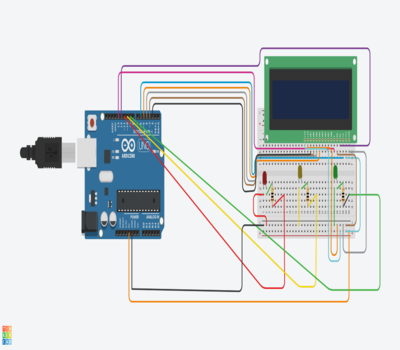
\includegraphics{ard.png}
    The Link of Tinkercad File : \href{https://www.tinkercad.com/things/hc84ooOnekb-cool-bigery-lahdi/editel?tenant=circuits}{Click Here}.
\end{figure}

\newpage
\subsection{\underline{Hardware Used}}
\begin{enumerate}
    \item Breadboard
    \item Jumper Wires
    \item Red LED
    \item Green LED
    \item Yellow LED
    \item  3 Resistors of 220 $\Omega$
    \item Arduino UNO
    \item LCD Screen
\end{enumerate}

\subsection{\underline{Arduino Code}}
\begin{lstlisting}[language=Arduino]
#include <LiquidCrystal.h>
int Contrast = 68;
LiquidCrystal lcd(12, 13, 5, 4, 3, 2);
const int redPin = 11;
const int yellowPin = 10;
const int greenPin = 9;
int brightness_1 = 0;
int fadeAmount_1 = 5;
int brightness_2 = 0;
int fadeAmount_2 = 5;
int brightness_3 = 0;
int fadeAmount_3 = 5;
bool val_1 = true;
bool val_2 = true;
bool val_3 = true;
char comdata;
void setup() {
  // put your setup code here, to run once:
  pinMode(redPin, OUTPUT);
  pinMode(greenPin, OUTPUT);
  pinMode(yellowPin, OUTPUT);
  analogWrite(6, Contrast);
  lcd.begin(16, 2);
  Serial.begin(9600);
  Serial.println("Press B to start the program");
  Serial.println("Then press R - RED ON, G - GREEN ON, Y -  YELLOW ON, r - TO RESET, X - ALL is OFF  ");
  Serial.print("choose the letter: ");
}

void loop() {
  // put your main code here, to run repeatedly:
  if (Serial.available() > 0) {
    comdata = char(Serial.read());
    if (comdata == 'R' || comdata == 'G' || comdata == 'Y' || comdata == 'X' || val_1 == true || val_2 == true || val_3 == true || comdata == 'B' || Serial.available() == 0) {
      if (comdata == 'B') {
        Serial.println("Your Program Has Started");
        lcd.setCursor(0, 0);
        lcd.print("Program Started");
      }
      else if (comdata == 'X') {
        Serial.println("ALL LEDs ARE OFF");
        digitalWrite(redPin, LOW);
        digitalWrite(greenPin, LOW);
        digitalWrite(yellowPin, LOW);
        lcd.setCursor(0, 0);
        lcd.clear();
        lcd.print("TURNED OFF");
      }
      while (comdata == 'R' || val_1) {
        if (comdata == 'R')
        {
          Serial.println("Red LED is ON");
          lcd.setCursor(0, 1);
          lcd.clear();
          lcd.print("RED LED IS ON");
        }
        analogWrite(redPin, brightness_1);
        brightness_1 = brightness_1 + fadeAmount_1;
        if (brightness_1 == 0 || brightness_1 == 255)
        {
          fadeAmount_1 = -fadeAmount_1;
        }
        delay(30);
        if (Serial.available() > 0)
        {
          digitalWrite(redPin, LOW);
          val_1 = !val_1;
          break;
        }
      }
      while (comdata == 'G' || val_2) {
        if (comdata == 'G')
        {
          Serial.println("Green LED is ON");
          lcd.setCursor(0, 1);
          lcd.clear();
          lcd.print("GREEN LED IS ON");
          //delay(2000);
        }
        analogWrite(greenPin, brightness_2);
        brightness_2 = brightness_2 + fadeAmount_2;
        if (brightness_2 == 0 || brightness_2 == 255)
        {
          fadeAmount_2 = -fadeAmount_2;
        }
        delay(30);
        if (Serial.available() > 0)
        {
          digitalWrite(greenPin, LOW);
          val_2 = !val_2;
          break;
        }
      }
      while (comdata == 'Y' || val_3) {
        if (comdata == 'Y')
        {
          Serial.println("Yellow LED is ON");
          lcd.setCursor(0, 1);
          lcd.clear();
          lcd.print("YELLOW LED IS ON");
          //delay(2000);
        }
        analogWrite(yellowPin, brightness_3);
        brightness_3 = brightness_3 + fadeAmount_3;
        if (brightness_3 == 0 || brightness_3 == 255)
        {
          fadeAmount_3 = -fadeAmount_3;
        }
        delay(30);
        if (Serial.available() > 0)
        {
          digitalWrite(yellowPin, LOW);
          val_3 = !val_3;
          break;
        }
      }
    }
    else
    {
      Serial.println("Please Use Above Mentioned KeyWords");
      lcd.setCursor(0, 1);
      lcd.clear();
      lcd.print("WRONG INPUT");
    }
  }
}
\end{lstlisting}

\newpage
\subsection{\underline{Brief Description}}
One of our motto of this project is to show the corresponding states in an LCD Screen.So, for that we need to call a library named : \textit{LiquidCrystal.h}
After that, we are assigning arduinos digital pins : $12, 13, 5, 4, 3, 2$ to lcd screen 
and Pin NO. 11, 10, 9 are assigned to respectively to RED, YELLOW,GREEN LED. For each LEDs brightness amount to 0 and fade amount to 5.
And 3 Boolean variables are declared  having TRUE. And another variable comdata of character datatypeis declared.

Then the arduino code is to setup with pin mode of respective LEDs  and lcd Screen needs to be started using \textit{lcd.begin()} function.
After that requirements to run the program is shown on the \textit{Serial Monitor} and user is asked to give input accordingly.
In the loop section we are going to check if user has given any input by the function \textit{Serial.available()} . If any value is available in the serial monitor then it is stored in comdata variable.

Then comdata value is checked with certain conditions that is if it is any of B, R, G, Y, X then we are entering the loop.
But the condition doesn't end here we need to check for the boolean values too and also if \textit{Serial.available()} is 0.We're going to enter the loop because for each turn Serial.available is going to be zero so the loop will break resulting shutting of the LED after one Fading-Glowing.

Now User can check if the program has started yet or not by inputting 'B'.
User can also turn off all the LEDs by giving 'X'.
And for the main part in a while loop weare going to check if comdata has value R, G or Y and with each of them their corresponding assigned boolean variables and that's how the loop doesn't stopped even if comdata has no value given.
\\
And with these piece of code :
\begin{lstlisting}[language=Arduino]
brightness = brightness + fadeAmount;
if (brightness == 0 || brightness == 255)
{
 fadeAmount = -fadeAmount;
}
\end{lstlisting}
we're actually controlling the brightness of the LED . These is the main logic that makes the LEDs behave like fading and brightenning continously.
Let's see what's the logic about:
\\
Initially our brightness variable has value 0. Now we are increasing it's value by fadeamount that is 5.As our brightness variable has now value 5 it doesn't enters the if condition. And it gets increased with 5 amount each time the loop runs. When the overall sum of brightness and fadeamount reaches 255 i.e.when brightness becomes 255 it finally satisfies the if condition loop and enters it. Here the sign of fade amount  gets changed . As a result fade amount is -5 now.and thus brghtness decreases by 5 amount and when itfinally reaches 0 it again satisfies the if condition and again enters the if and our fade amount's sign gets changed . So, it's +5 again and the first process of glowing the LED occurs nad it repeats infinitely . So, now we need to stop this loop. And for that:
\begin{lstlisting}[language=Arduino]
if (Serial.available() > 0)
{
 digitalWrite(LEDPin, LOW);
 val = !val;
 break;
}
\end{lstlisting}
Within that while loop another if condition is introduced to check if user has given any input or not.And if any input is available this above mentioned condition gets satisfied and using \textit{digitalWrite()} the used LED is stopped i.e. turns into low and our boolean value is reversed and thus the loop gets broken.


\section{Results and Discussion}
Our program looks so far so good it works fine. But I need to mention two points firstly when I wrote the code for the first time I decided to write using a for loop inside a if condition but while dealing with it I noticed that it stops after completing a full cycle of glowing-fading.And that is because when next time it starts running our serial.available is null then so it doesn't fullfill our condition and hence stops working.Then after a quite bit of thinking i changed my way of aproaching the problem and rather using if then for I used a if statement to check if comdata has desired values or its null thats ow I overcame the problem of running the program for second time . But the problem doesn't ends here.Now i need a while loop to make the led to glow-fade infinitely.Then I thought inside while if I check only a particular condition that is not going to give me an infinite loop. Then an idea struck my mind few days before I was working on a Python Project of creating a snake game there I used a infinite while loop that checks if a varable has the boolean value true or not and inside that loop i used functions to detect if that snake has collided with a food or collided with itslef or hits the wall and increase it's length and I assign that variable to False when it's satisfies certain condition.And that's how I came up with the idea of using a boolean variable to check along with the previous condition. Now, one can ask that we could also use the condition that is $ series.available == 0 $ but the problem is then after completing a cycle our program will be confused because the same condition will be used for Red, Green, Yellow LED too. So, we simple can't use that .
And then after reading the question again I realized that it is not mentioned clearly that the LED is needed to glow-fade continously then I consullted our H.O.D S.S.B sir what should I do? then he suggested to go with the latter and keep the loop running unless another input is given by the User. Felt kinda releived I didn't waste my time. Then sir suggested I should do something when the user gives some invalid input.So, Sir kind of did the debugging of my code on his own. Then I implimented a simple else statement corresponding to the if statement where I checked if user has given certain inputs oor not. And then some tuning My code was ready to go . After that I thought why not use an LCD screen too to show corresponding outputs for each condition.For that I did quite a digging through internet because I had no idea how to use LCD . there in that instance I faced some debugging issues and finally finished this programming.
\\
And I specially want to mention that while writting the PDF in \text{A\LaTeX\ } I faced an issue to use the arduino code . After quite digging I found a github file that allows arduino code to write in latex without any external problem and I used that. But I noticed maybe the code is written in certan way that in my print statements in arduino code the space between words filled by a weird shaped character. I tried to remove that but I  dont know how to interact with the mother file. So,I'm keeping it untouched like this.
\section{Conclusion}
In conclusion, Our project \textit{"Fading-GLowing Of LEDs"} has been successfully made using some simple codes to control the LEDs.We finally achieve all of our goals . After running the program we can see in serial monitor that it is asking for inputs from user. After we press B it represents that the program is running and corresponding message is shown in both serial monitor and in lcd screen.
After that let's assume user presses R which represents Red LED , red led  starts glowing then fading and vice versa repeatedly untill and unless user interrupts it with another input . If that another input is G or Y or X it executes the corresponding task i.e on pressing G or Y it glows-fades just like previously mentioned.and on pressing X LED glowing-fading stops.Let's assume user gives some another input in that case Serial monitor and lcd screen shows to give only mentioned inputs by program.

\section{Acknowledgement}
I would like to express my special thanks of gratitude to our Physics Department H.O.D S.S.B Sir who gave me the golden opportunity to do this wonderful project on the topic \textit{Arduino project of Controlling LED's using serial monitor}, which also helped me in doing a lot of Research and i came to know about so many new things I am really thankful for that.
Secondly i would also like to thank my parents and friends who helped me a lot in finalizing this project within the limited time frame.

\begin{thebibliography}{}
\bibitem{github}
Github Repo of trihedral (Kyle). It solved the issue of using arduino code directly in \text{\LaTeX\ } .
\href{https://github.com/trihedral/ArduinoLatexListing}{Click Here}.

\bibitem{arduino}
Official Arduino Site of query of how to clear LCD Screen.
\href{https://www.arduino.cc/en/Reference/LiquidCrystalClear}{Click Here}.

\end{thebibliography}
\end{document}

